\documentclass[a4paper,12pt]{article}
\usepackage{graphicx}
\usepackage{geometry}
\usepackage{titling}
\usepackage{fancyhdr}
\usepackage{lmodern}
\usepackage{setspace}
\usepackage{datetime}
\usepackage{tocloft}
\usepackage{siunitx}
\usepackage{tcolorbox}

% Page Setup
\geometry{margin=1in}
\setlength{\parindent}{0pt}
\setlength{\parskip}{1em}

% Header & Footer
\pagestyle{fancy}
\fancyhf{}
\fancyhead[L]{Powertrain}
\fancyhead[R]{TLS’e Racing}
\fancyfoot[R]{\thepage}


\usepackage{subcaption}
\usepackage{float}

% Figures path
\graphicspath{{../Images/}}


\begin{document}

% Title Page
\begin{titlepage}
    \centering
    \vspace*{1cm}
        
        % Logo
        
\includegraphics[width=1\textwidth]{Logo TLS'e.png} % Replace with your actual logo file
        
        \vspace{1.5cm}
        
        % Title with horizontal rules
        \hrule
        \vspace{0.4cm}
        {\Large\bfseries Battery container simulation on Ansys \par}
        \vspace{0.4cm}
        \hrule
        
        \vspace{1.5cm}
        
        % Subtitle
         \Large
        Division: Powertrain\\
        Author: Friedly WOLI \\
        \vspace{0.5cm}
        
        % Season
        \textbf{Season 2025-2026}
       
        \vfill
        \today

        \normalsize
         Version: 1.0
    
        \vspace{0.5cm}
        \textit{This document is confidential and intended for internal use only.}
        
\end{titlepage}

\newpage
\tableofcontents
\newpage

\section{\textcolor{red}{Introduction}}
\label{sec:Introduction}

This section presents the finite element analysis (FEA) of a battery container performed using Ansys Mechanical. The objective is to evaluate the structural response of the container under realistic loading conditions, including gravity and acceleration.

\vspace{2cm}

\section{\textcolor{red}{Rules and Regulations}}
\label{sec:Rules and Regulations}

%--------------------------------------------------
%--------------------------------------------------


The TSAC structure, its mounting to the chassis, and the internal mounting of every cell must withstand the following inertial accelerations simultaneously or in independent load cases as specified in the ASES \\ $ Rule: T9.2.1 $:
\begin{itemize}
	\item \textbf{Longitudinal Direction (Forward/Aft):} $40\,g$
	\item \textbf{Lateral Direction (Left/Right):} $40\,g$
	\item \textbf{Vertical Direction (Up/Down):} $20\,g$
\end{itemize}

\subsection{Segment and Mass Constraints}
Each individual accumulator segment within the container must respect the following limits :\\
$ Rule: EV5.3 $
\begin{itemize}
	\item \textbf{Maximum Mass:} $12\,\text{kg}$
	\item \textbf{Maximum Static Voltage:} $120\,\text{VDC}$
	\item \textbf{Maximum Energy:} $6\,\text{MJ}$
\end{itemize}

\subsection{Material Baseline Thicknesses}
If metallic materials are used, the following minimum thicknesses must be respected to avoid further equivalency proofing. Any thickness below these requires simulation/testing data in the ASES :


\begin{tabular}{|l|c|r|}

	\textbf{Component} & \textbf{Steel (Min)} & \textbf{Aluminium (Min)} 	\\ 
	Container Bottom   & $1.25\,\text{mm}$    & $3.2\,\text{mm}$        	\\
	Vertical Walls     & $0.9\,\text{mm}$     & $2.3\,\text{mm}$        	\\
	Lid and Covers     & $0.9\,\text{mm}$     & $2.3\,\text{mm}$        	\\ 
	
\end{tabular}


\subsection{Structural Geometry Rules}
\begin{itemize}
	\item \textbf{Internal Walls:} Segments must be separated by internal vertical walls that extend upwards until the lid .
	\item \textbf{Cutouts/Holes:} The total cutout area (for cooling or wiring) must be \textbf{less than 25\%} of the area of the respective single wall.
	\item \textbf{Pouch Cell Fixation:} Pouch cells must be fixed on at least \textbf{80\%} of their large surfaces.
\end{itemize}

\subsection{Simulation Environment and Fasteners}
\begin{itemize}
	\item \textbf{Ambient Temperature:} For non-metallic materials (excluding continuous fiber laminates), calculations must assume \textbf{$60\,^\circ\text{C}$} .
	\item \textbf{Attachment Points:} A minimum of \textbf{2 attachment points} to the chassis is required .
	\item \textbf{Mounting Brackets:} Must be steel ($\ge 1.6\,\text{mm}$) or aluminium ($\ge 4\,\text{mm}$) with gussets for bending loads .
	\item \textbf{Edge Distance (e/D):} All bolted joints must respect an edge distance ratio of \textbf{$1.5$} or greater .
\end{itemize}



%--------------------------------------------------
%--------------------------------------------------

\vspace*{2cm}


% ==================================================
\section{ \textcolor{blue}{Assumptions, Methodology} }
% ==================================================

\begin{itemize}
	\item The battery modules are modeled as simplified rectangular volumes.
	\item The cells inside each module are not modeled individually.
	\item Each module is assigned an equivalent material with a density computed as:
	\[
	\rho = \frac{m_{\text{cells}}}{V_{\text{module}}}
	\]
	\item The weight of the cells is represented using distributed mass and gravity.
	\item Contact between modules and the container is simplified (bonded assumption).
\end{itemize}

\vspace*{2cm}

% ==================================================
\section{\textcolor{blue}{Implementation}}
% ==================================================

	
	% ==================================================
	\subsection{Geometry}
	% ==================================================
	
		\begin{itemize}
			\item The geometry is designed in Onshape and imported into Ansys.
			\item Container dimensions: \(590 \times 670 \times 270 \, \text{mm}\)
			\item Module dimensions: \(190 \times 371 \times 84.7 \, \text{mm}\)
			\item Spacing between modules: \(32.741 \, \text{mm}\)
			\item All components are modeled as rectangular prisms.
			
		\end{itemize}
		
		
		
		
		\begin{figure}[H]
			\centering
			
			\begin{subfigure}{0.45\textwidth}
				\centering
				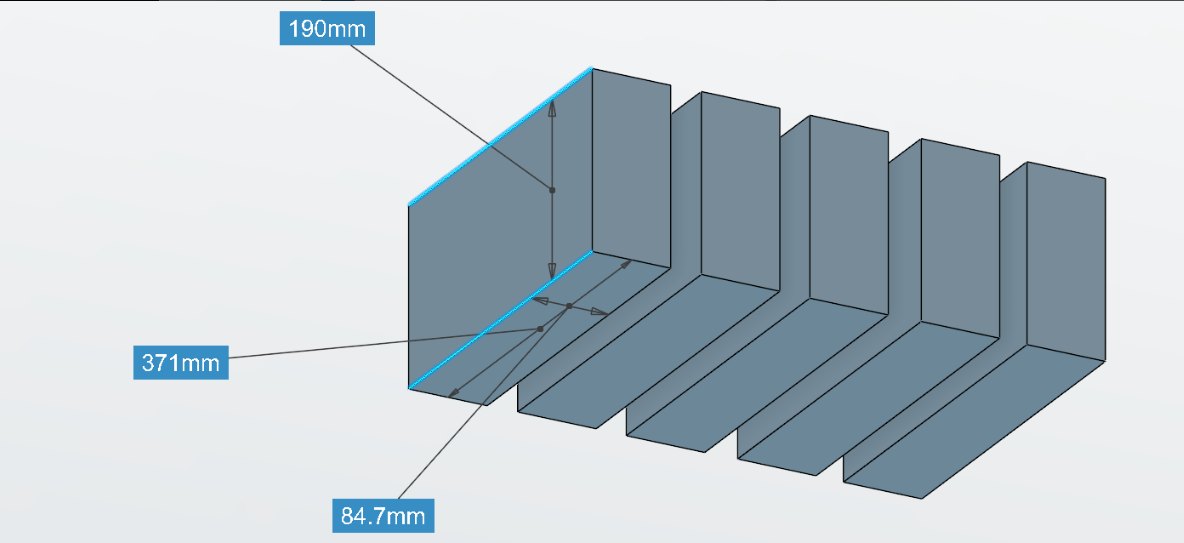
\includegraphics[width=\textwidth]{module_dimension.png}
			%	\caption{Première image}
			\end{subfigure}
			\hfill
			\begin{subfigure}{0.45\textwidth}
				\centering
				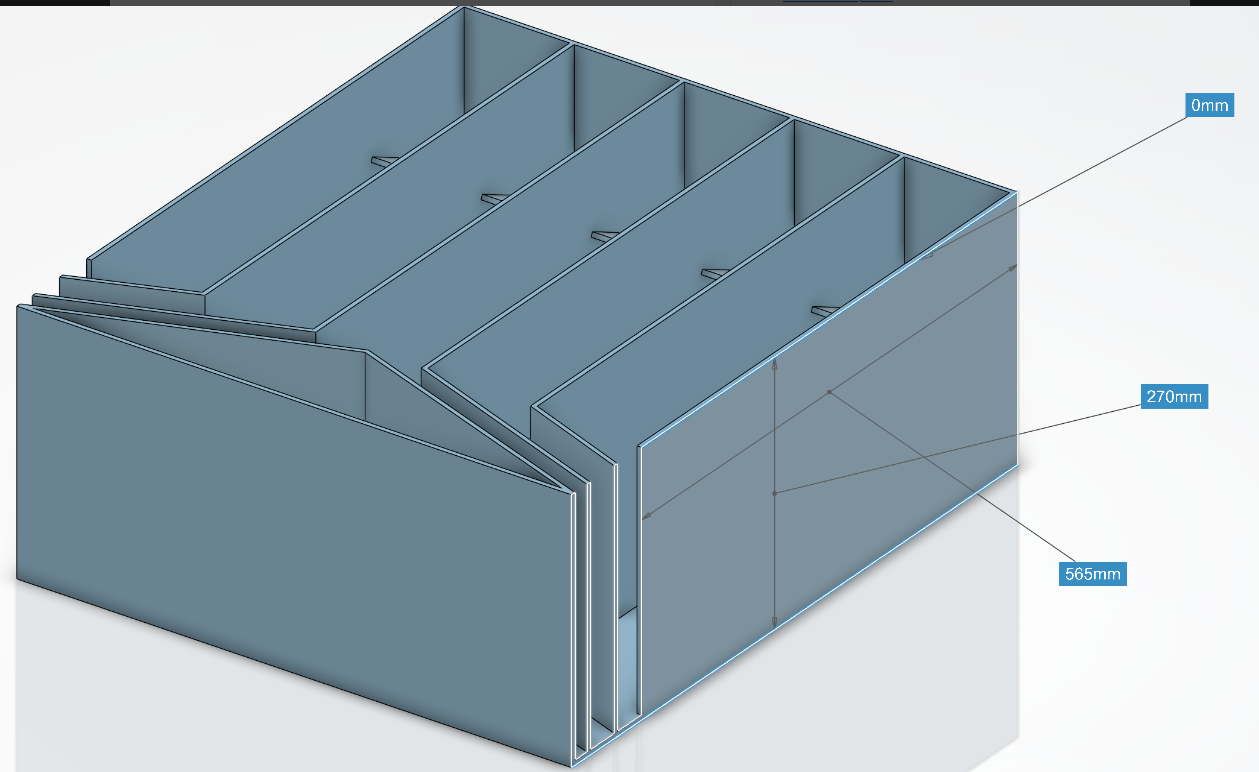
\includegraphics[width=\textwidth]{containeur_dimensions.png}
			%	\caption{Deuxième image}
			\end{subfigure}
			
			\caption{Shapes}
			\label{fig:double}
		\end{figure}
	
	% ==================================================
	\subsection{Material Characteristics}
	% ==================================================
	
		The container is made of aluminum to ensure realistic stiffness and strength behavior.
		
		\begin{figure}[H]
			\centering
		%	\includegraphics[width=0.7\textwidth]{Aluminum.png}
			\caption{Material properties of aluminum}
			\label{fig:material}
		\end{figure}
		
		
		The modules are assigned an equivalent material based on their density. A material close to this density is selected. In this case, Balsa wood is used with:
		\[
		\rho = 254 \, \text{kg/m}^3
		\]
		
		\begin{figure}[H]
			\centering
		%	\includegraphics[width=0.7\textwidth]{boxes-material.png}
			\caption{Material properties of aluminum}
			\label{fig:material}
		\end{figure}
	
	
	
	
	% ==================================================
	\subsection{Connexion}
	% ==================================================
	
		\subsubsection{Contact}
		
		The contact is modeled between each module and its corresponding surface on the battery container.  
		The type of contact is \textbf{Bonded} because:
		
		\begin{itemize}
			\item The module is directly screwed to the container.
			\item There is no gap between the module and the bottom surface.
			\item There is no sliding between the surfaces.
			\item The load is transferred through contact pressure.
		\end{itemize}
		
		\begin{figure}[H]
			\centering
			%\includegraphics[width=0.7\textwidth]{pressure_on_bottom_surface.png}
			\caption{Connection between module and container}
			\label{fig:pressure}
		\end{figure}
		
	
	
	% ==================================================
	\subsection{Loading and Boundary Conditions}
	% ==================================================
	
		\subsubsection{Gravity and Mass Representation}
		
		The mass of the cells is represented using a distributed mass applied to the module regions.
		
		Gravity is applied as follows:
		\begin{itemize}
			\item Direction: \(-Z\)
			\item Magnitude: \(9.81 \, \text{m/s}^2\)
		\end{itemize}
		
		This approach ensures that the weight of the cells is naturally transferred to the bottom surface of the container.
		
		\begin{figure}[H]
			\centering
			%\includegraphics[width=0.7\textwidth]{pressure_on_bottom_surface.png}
			\caption{Load transfer to the bottom surface}
			\label{fig:pressure}
		\end{figure}
		
		\subsubsection{Fixed Supports}
		
		Fixed supports are applied to represent the attachment of the container to the vehicle structure:
		\begin{itemize}
			\item Along the upper mounting edges
			\item On selected bottom regions \\ \\
		\end{itemize}
		
		
		
		\begin{figure}[H]
			\centering
			
			\begin{subfigure}{0.45\textwidth}
				\centering
				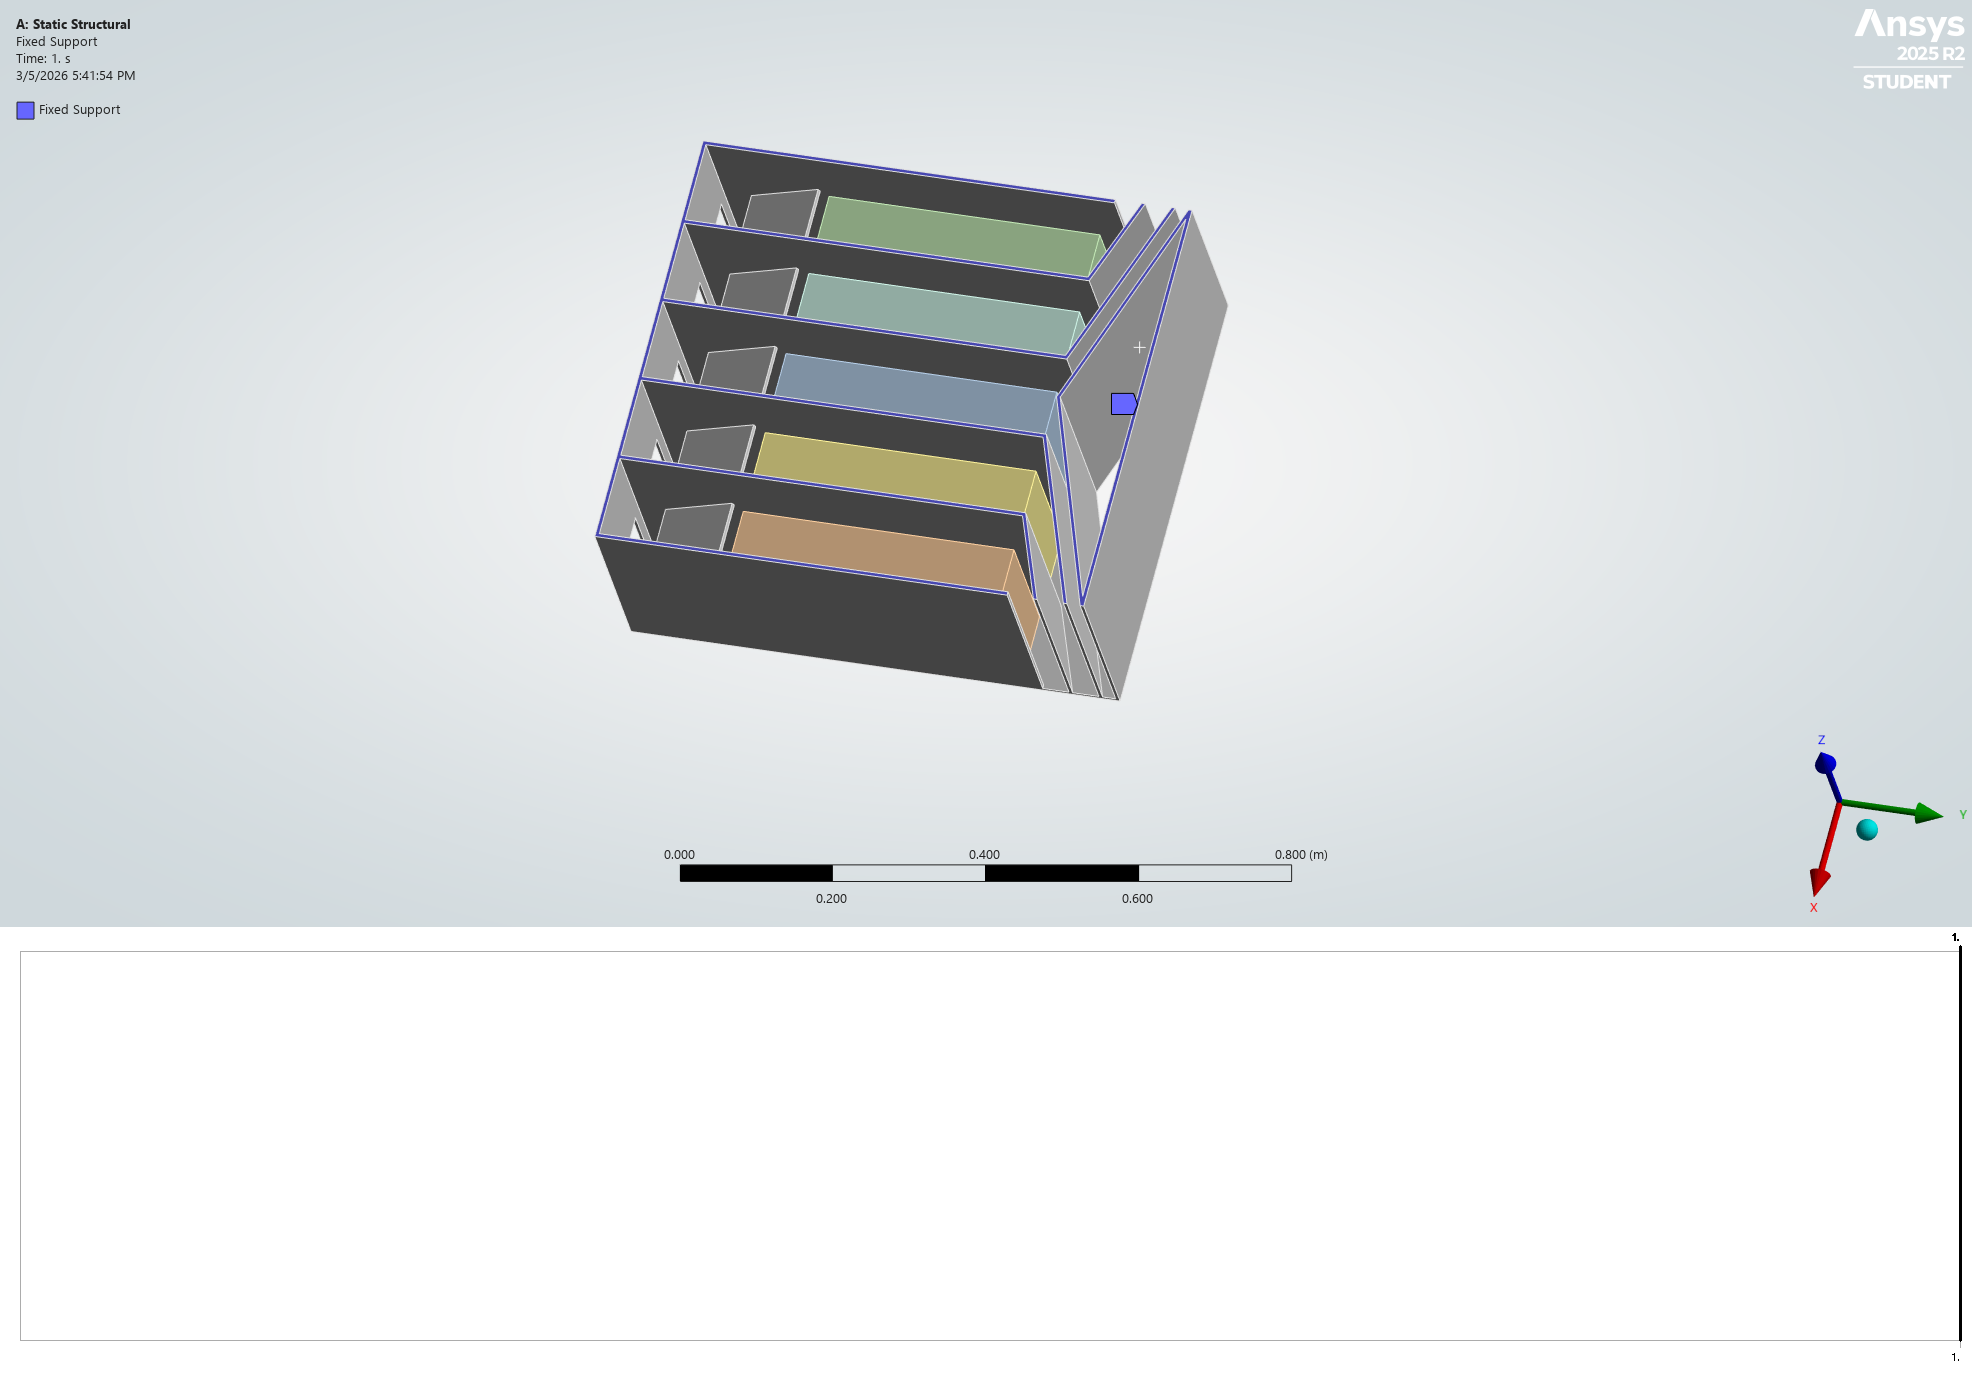
\includegraphics[width=\textwidth]{fixed-part.png}
			%	\caption{Première image}
			\end{subfigure}
			\hfill
			\begin{subfigure}{0.45\textwidth}
				\centering
				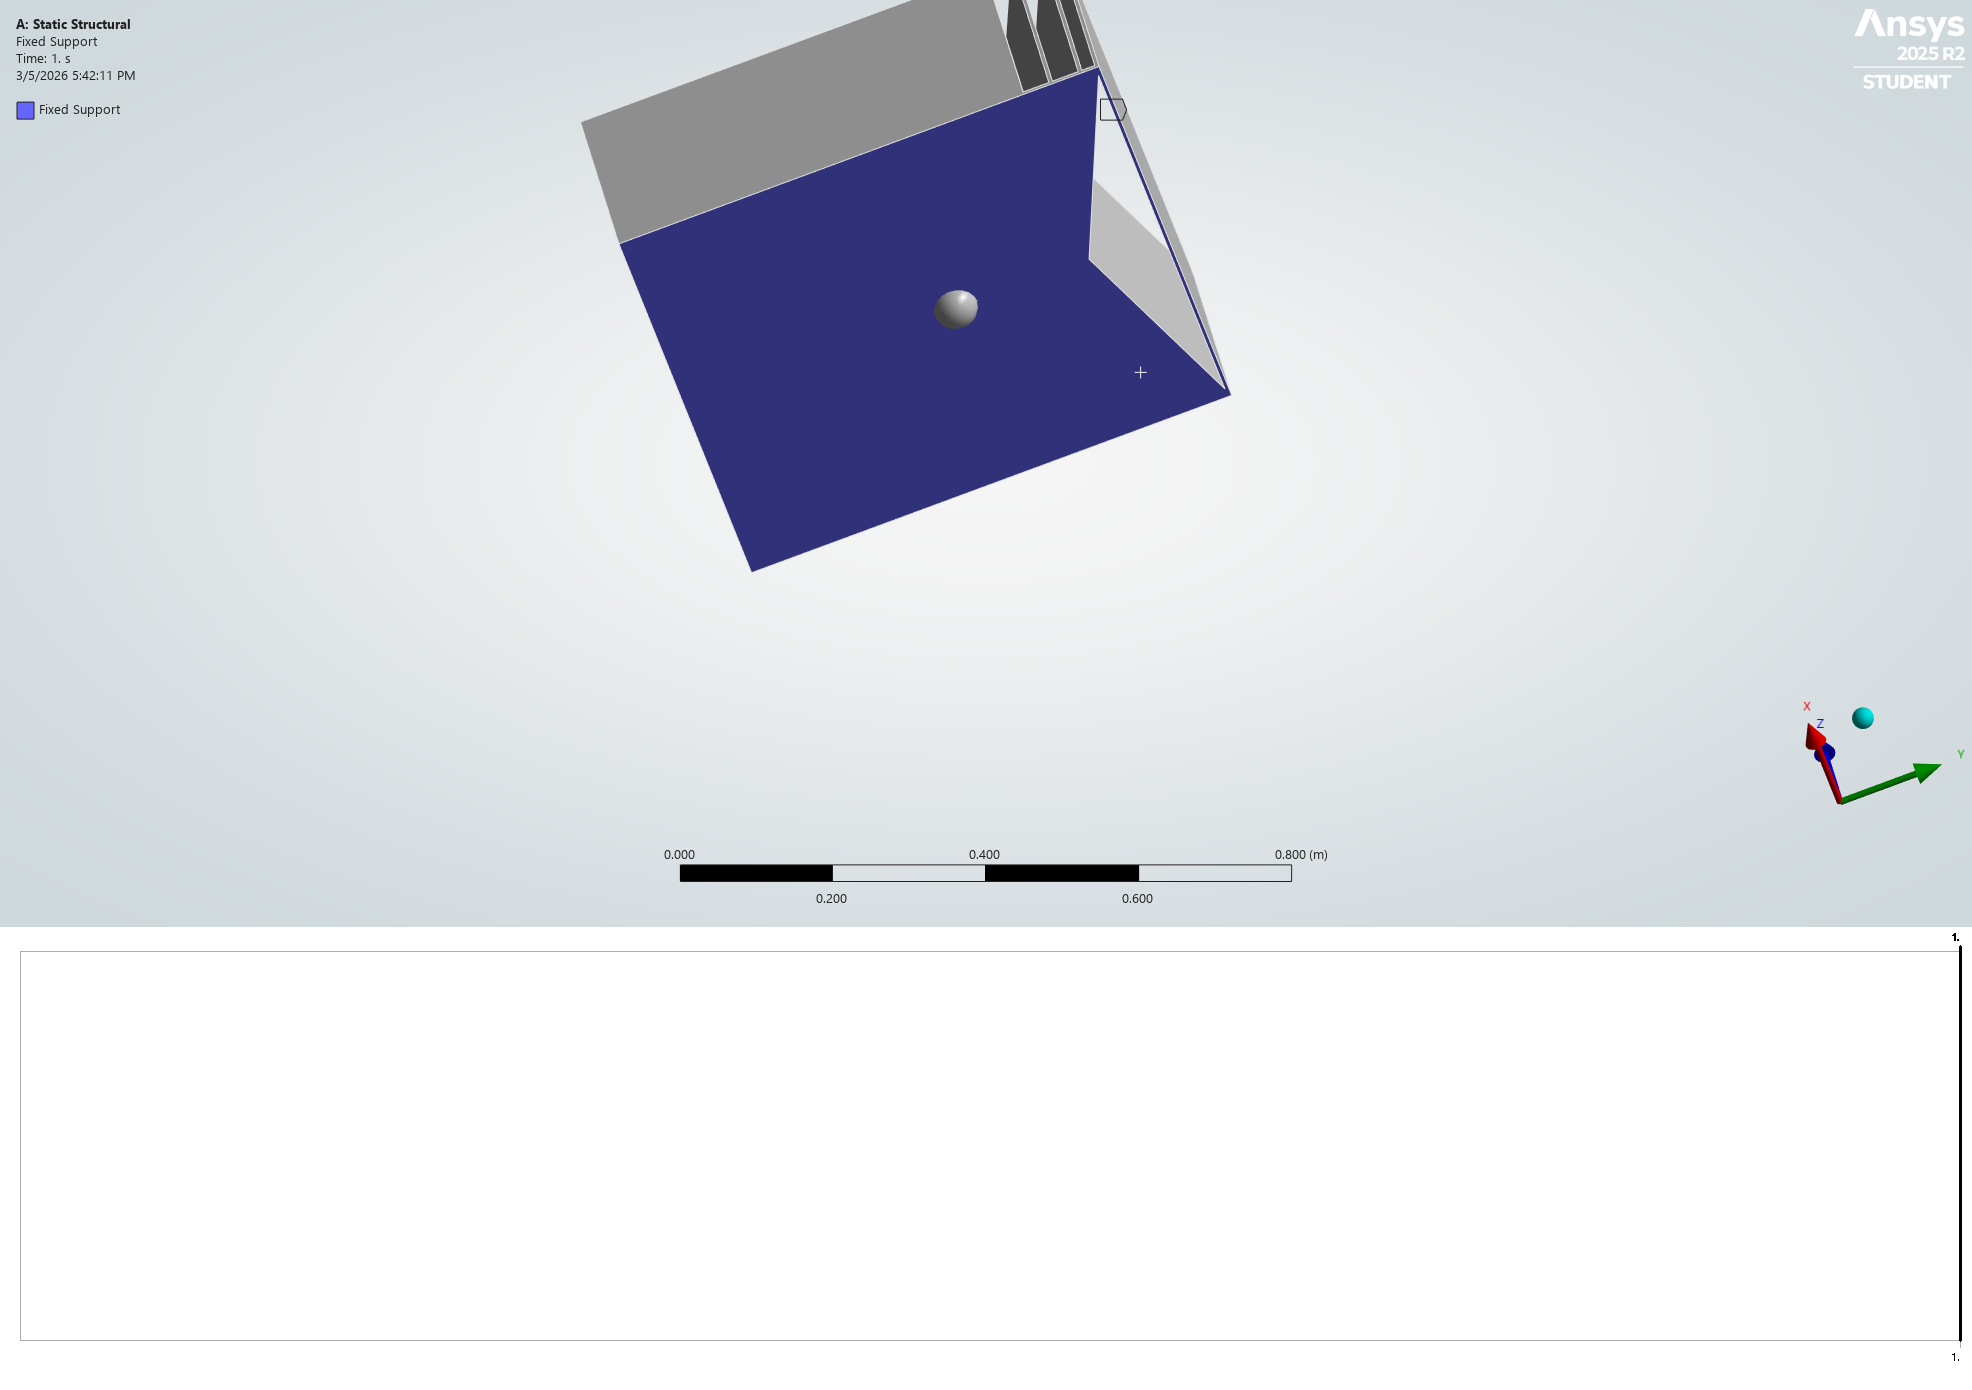
\includegraphics[width=\textwidth]{fixed-part1.png}
			%	\caption{Deuxième image}
			\end{subfigure}
			
			\caption{Boundary conditions (fixed supports)}
			\label{fig:double}
		\end{figure}
		
		
		
		\subsubsection{Acceleration Loads}
		
		Acceleration loads are applied to simulate extreme operating conditions:
		
		\begin{itemize}
			\item \(40g\) in the longitudinal direction (\(x\))
			\item \(40g\) in the lateral direction (\(y\))
			\item \(20g\) in the vertical direction (\(z\))
		\end{itemize}
		
		% ==================================================
		\subsection{Meshing Strategy}
		% ==================================================
		First simulation is done with  the default meshing
		A refined mesh is applied in critical areas, especially on the bottom surface where stress concentrations are expected.
		
		\begin{itemize}
			\item Element size on bottom surface: \(0.01 \, \text{m}\)
		\end{itemize}
		
		\begin{figure}[H]
			\centering
			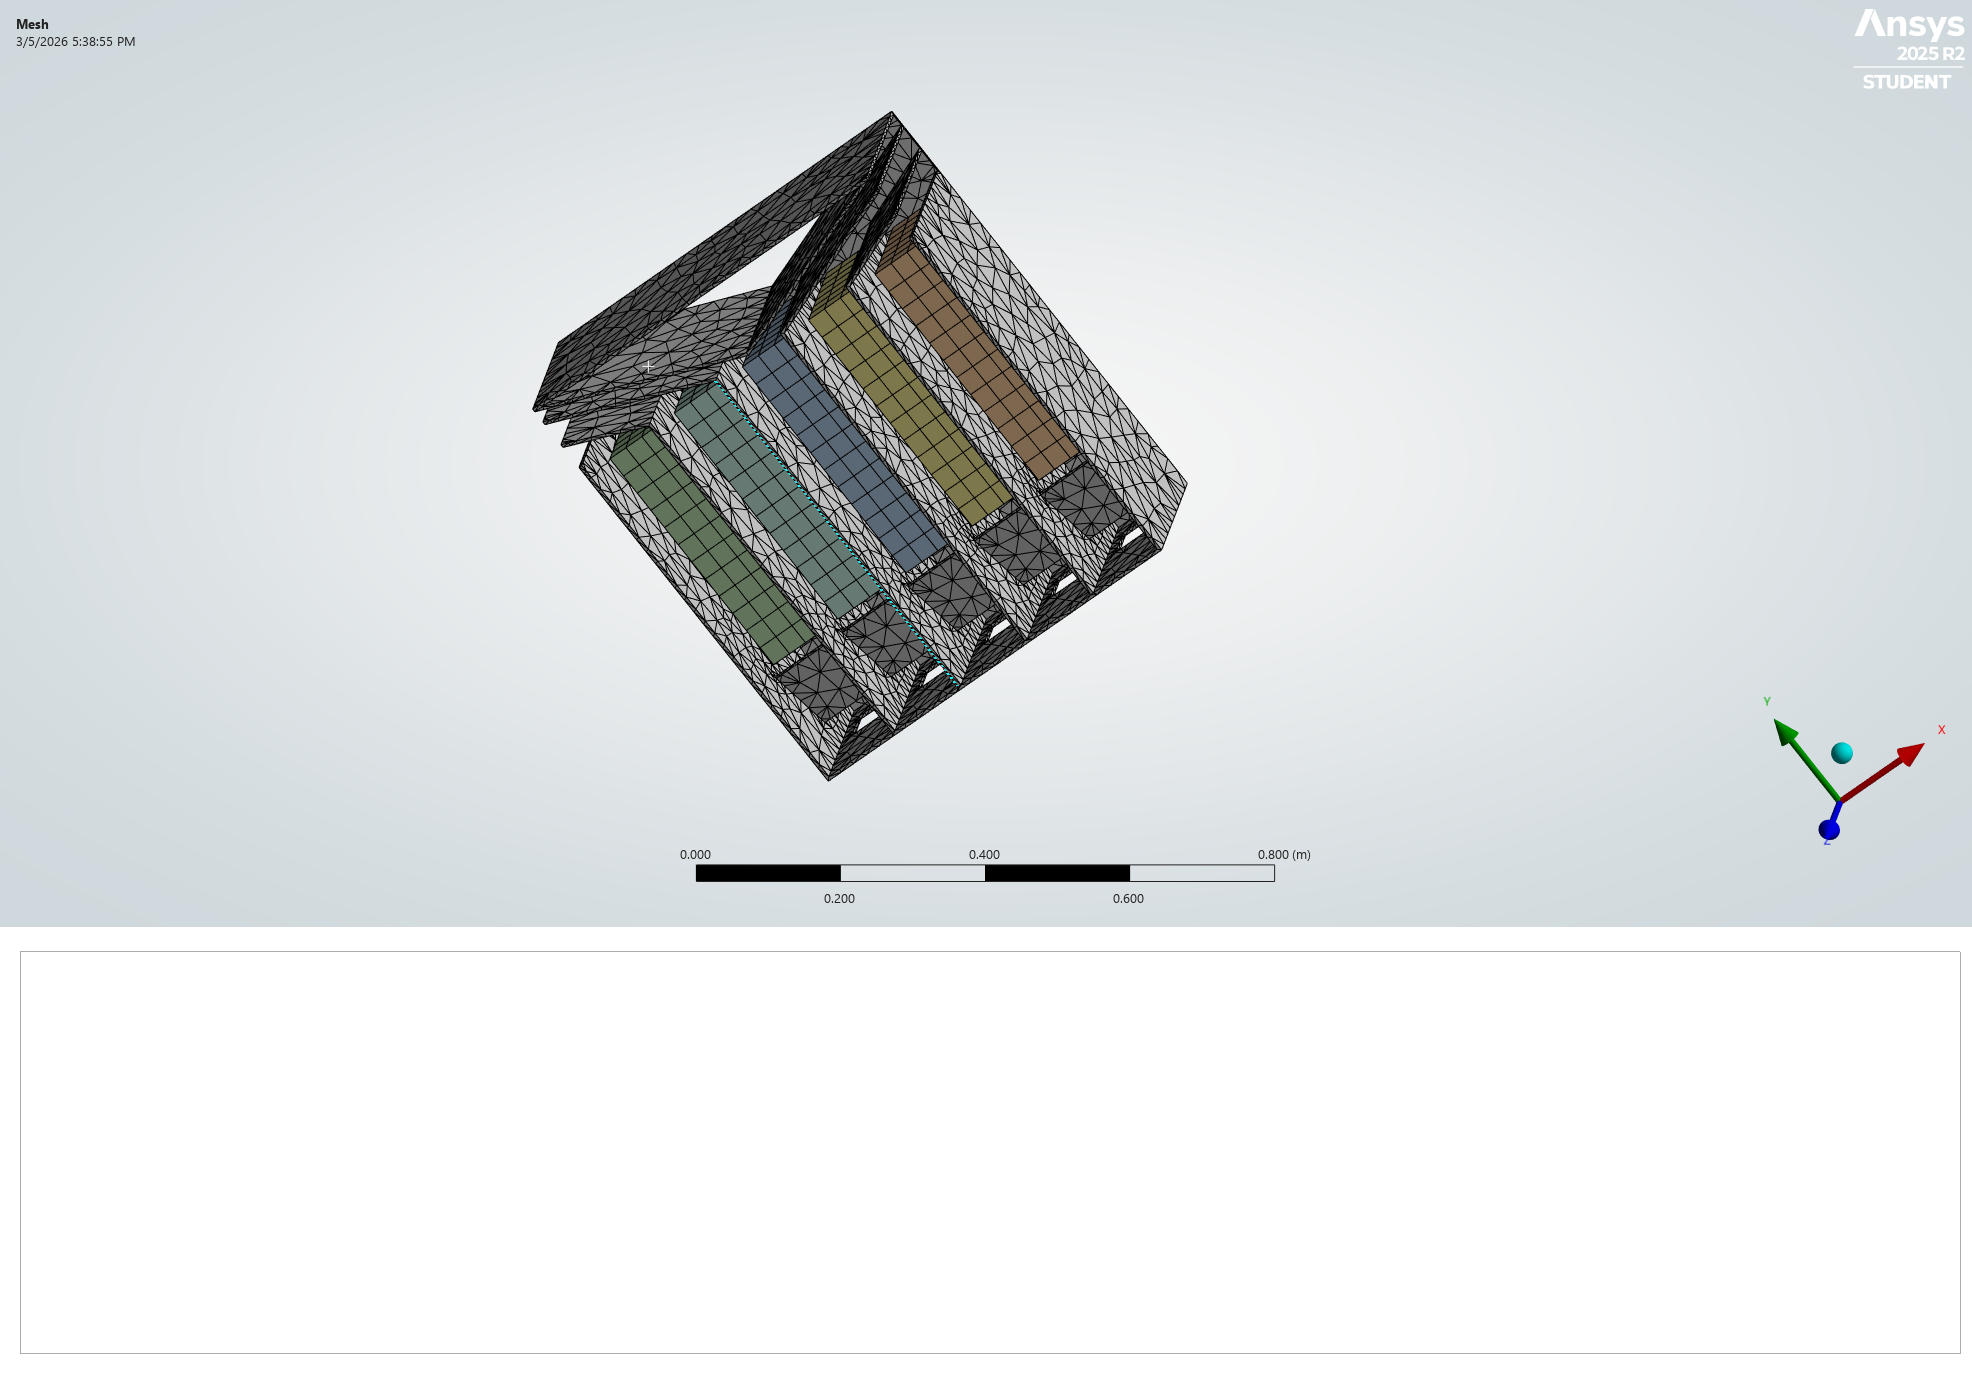
\includegraphics[width=0.7\textwidth]{meshing-by-default.png}
			\caption{Mesh configuration}
			\label{fig:mesh}
		\end{figure}













% ==================================================
\section{ \textcolor{blue}{Results}}
% ==================================================

\subsection{Total Deformation}
The total deformation highlights the global stiffness of the structure, with maximum deformation occurring in unsupported regions.  \\
The maximum deformation is $9.23 \times 10^{-6}$ m ($9.23~\mu$m), which is acceptable for this application.  
For acceleration along the x-direction, deformation occurs primarily on the lateral side. In reality, this lateral side will be maintained fixed by connection to another component, so this aspect requires further detailed study.

\begin{figure}[H]
	\centering
%	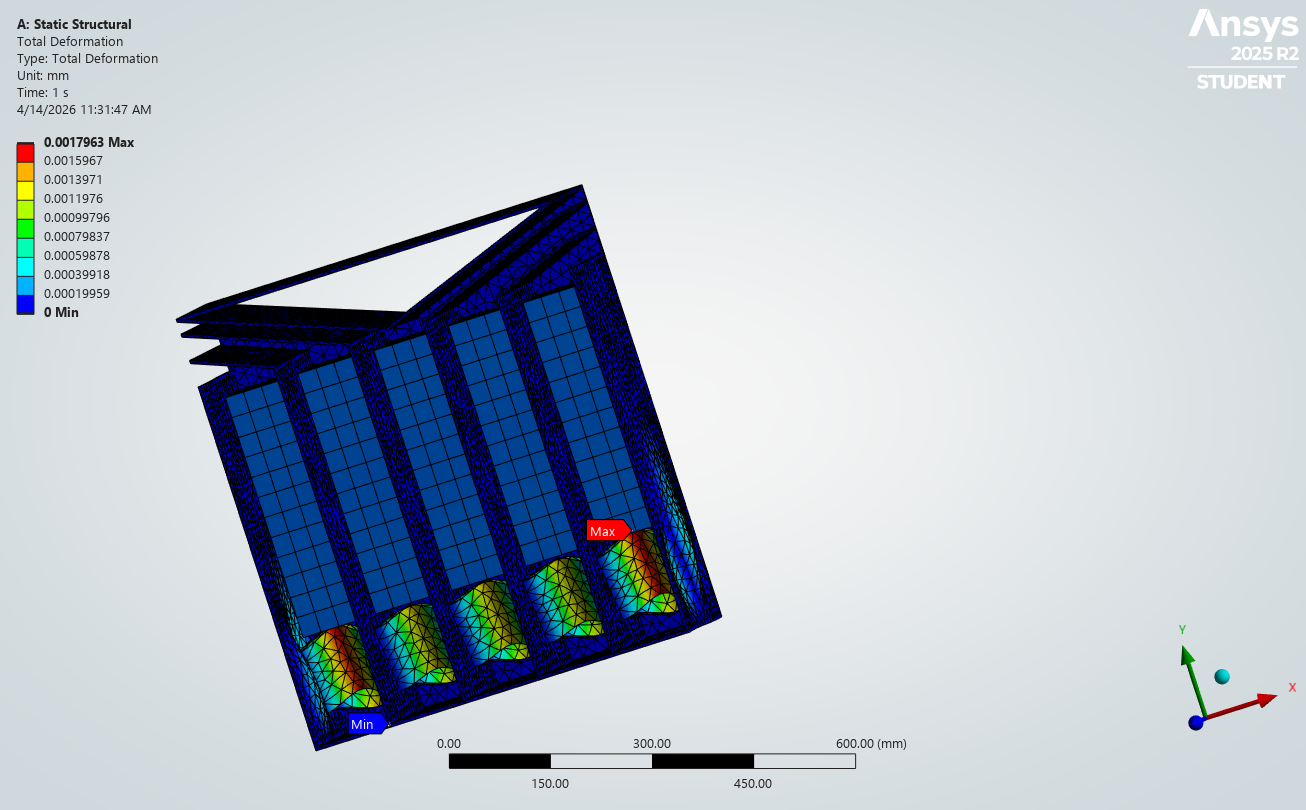
\includegraphics[width=0.7\textwidth]{Total_deformation.png}
	\caption{Total deformation}
	\label{fig:deformation}
\end{figure}

\subsection{Directional Deformation}


This is a useful plot because it shows the deformation along the X axis, not just the total displacement. The values are very small, from about -0.000503 mm to +0.000503 mm, so the part is only moving slightly in the global X direction

\begin{figure}[H]
	\centering
%	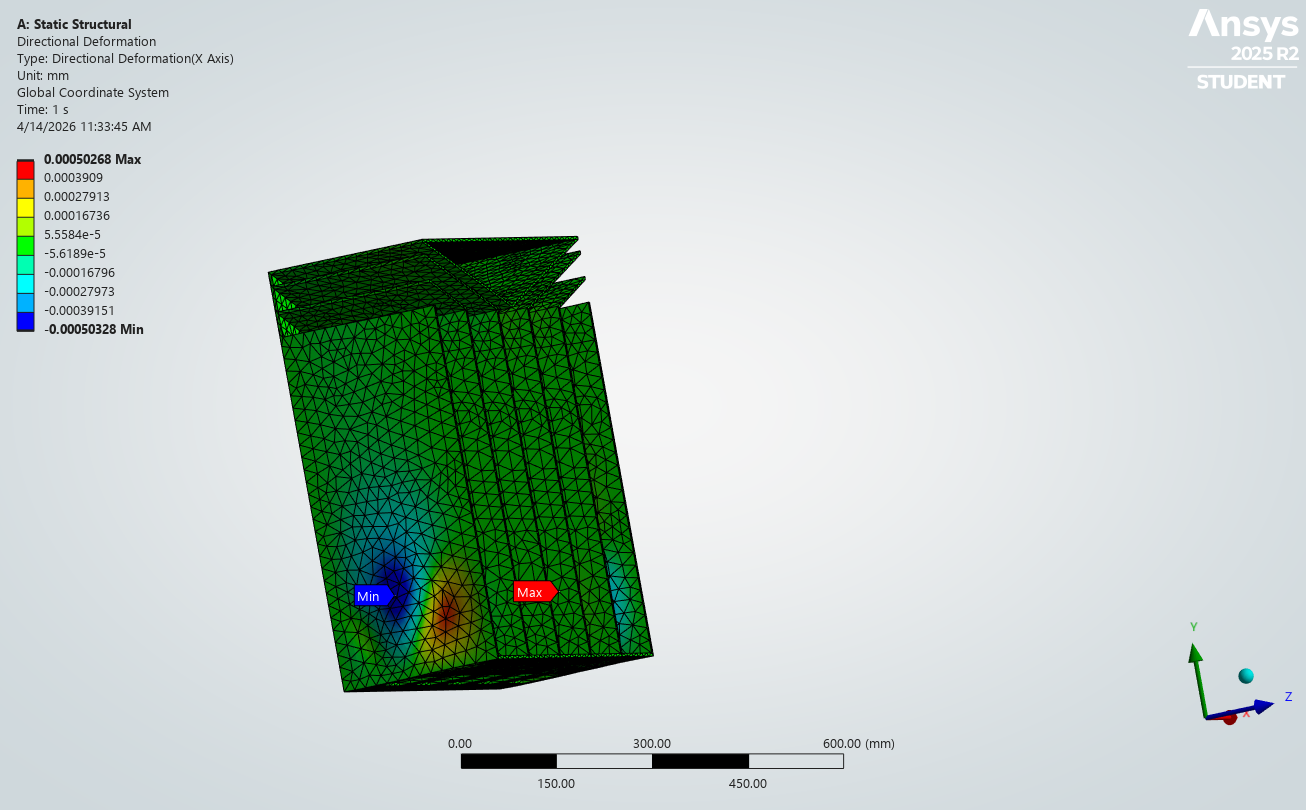
\includegraphics[width=0.7\textwidth]{directionnal_deformation.png}
	\caption{Directional deformation}
	\label{fig:dir_deformation}
\end{figure}

\subsection{Equivalent (Von Mises) Stress}

This equivalent von Mises stress result looks very low overall: the legend shows a maximum of about 0.36969 MPa and a minimum near zero, so the part is far from yielding.
Because the peak stress is only around 0.37 MPa and the fact that the material is aluminum the model is in a very safe elastic range 

\begin{figure}[H]
	\centering
%	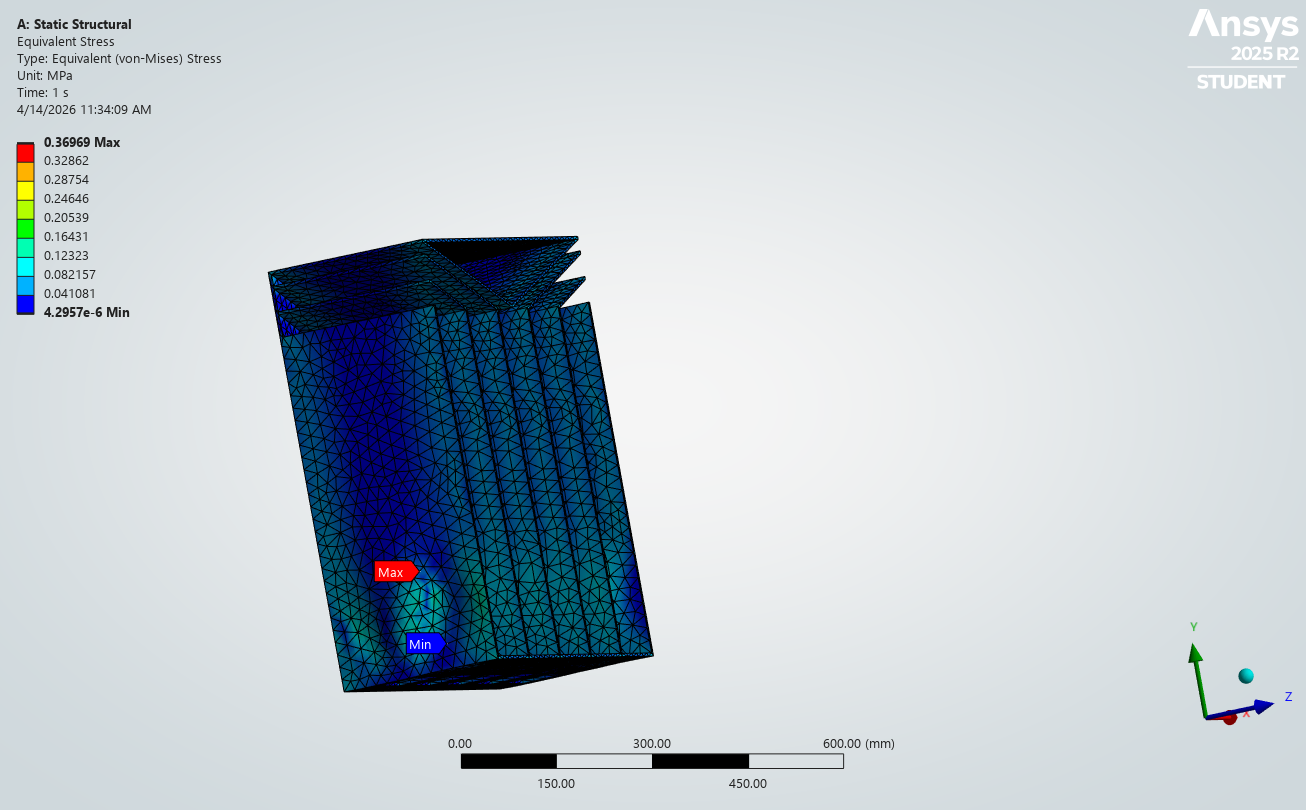
\includegraphics[width=0.7\textwidth]{equivalent_stress.png}
	\caption{Equivalent (Von Mises) stress}
	\label{fig:stress}
\end{figure}









\vspace*{2cm}
% ==================================================
\section{ \textcolor{blue}{Discussion and Analysis}}
% ==================================================


\label{sec:Discussion and Analysis}
Discuss the significance of the results. Consider:
\begin{itemize}
    \item Comparison with expected outcomes
    \item Challenges encountered
    \item Possible improvements
\end{itemize}













\vspace*{2cm}

% ==================================================
\section{\textcolor{red}{Conclusion}}
% ==================================================

\label{sec:Conclusion}

The overall results are good since the deformations are very low. The results also fit well with the characteristics of aluminum. For a more accurate simulation, we will modify the surface of the module in contact with the bottom surface of the container to improve the transmission of forces between the two parts.




\section{Cost and Manufacturing}
\label{sec:Cost and Manufacturing}
Present the estimated costs and manufacturing considerations, provide background on the chosen production methods and materials, and explain how these factors influence the project’s feasibility, efficiency, and overall quality.

\section{Future Work}
\label{sec:Future Work}
Outline potential next steps, future improvements, or additional research required.

\section{References}
\label{sec:references}
Use the following format for citations:
\begin{itemize}
    \item \texttt{\textbackslash cite\{authorYear\}} for in-line citations
    \item List all references in BibTeX format at the end
\end{itemize}

%\bibliographystyle{plain}
%\bibliography{references}

\end{document}

% Note that this report must be submitted with each part and assembly you do.
% The report and part/assembly CAD must be submitted to the scrum with an excel sheet of the Cost and Manufacturing of the part/assembly.
% Each part designed must have its own CBOM.
% Each assembly made must have its own DBOM.